\documentclass{article}
\usepackage{hyperref}
\usepackage{listings}
\usepackage{color}
\usepackage{geometry}
\usepackage{graphicx}
\usepackage{amsmath}
\usepackage{caption}
\usepackage{subcaption}
\geometry{margin=1in}
\pdfminorversion=6

\newcommand\TODO[1]{\textcolor{red}{TODO: #1}}

\newcommand\header[2]{
    \begin{center}
        {\large
        UCSD CSE 272 Assignment #1: \\
        \vspace{0.3cm}
        \Large
        #2}
    \end{center}
}

\definecolor{dkgreen}{rgb}{0,0.6,0}
\definecolor{gray}{rgb}{0.5,0.5,0.5}
\definecolor{mauve}{rgb}{0.58,0,0.82}
\lstset{frame=tb,
        aboveskip=3mm,
        belowskip=3mm,
        showstringspaces=false,
        columns=flexible,
        basicstyle={\small\ttfamily},
        numbers=none,
        numberstyle=\tiny\color{gray},
        keywordstyle=\color{blue},
        commentstyle=\color{dkgreen},
        stringstyle=\color{mauve},
        breaklines=true,
        breakatwhitespace=true,
        tabsize=2
}


\begin{document}

\header{2}{Volumetric Path Tracing (tentative draft)}

\begin{figure}[h]
    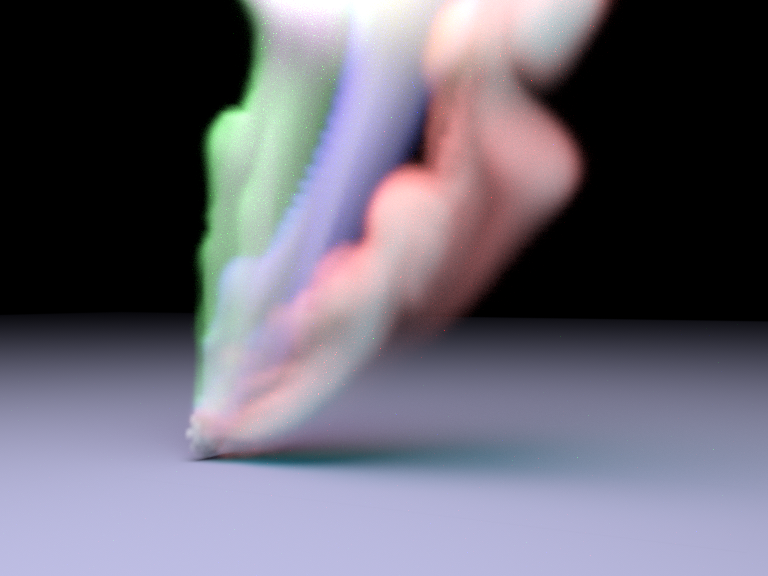
\includegraphics[width=\linewidth]{imgs/colored_smoke.png}
    \caption{A heterogeneous volume with spectrally varying density over space, rendered with multiple-scattering. Smoke data are generated using Wenzel Jakob's \href{http://www.mitsuba-renderer.org/misc.html}{fsolver}.}
    \label{fig:gallery}
\end{figure}

In this homework, we will build a volumetric path tracers that can handle scattering and absorption inside participating media inside lajolla. We will split the development into 6 steps and build 6 volumetric path tracers, each has more features than the previous ones.\footnote{This approach is inspired by Steve Marschner's \href{https://www.cs.cornell.edu/courses/cs6630/2015fa/notes/10volpath.pdf}{course note} on volumetric path tracing.} Your $n$-th volumetric path tracer should be able to render all scenes the $(n-1)$-th one can handle. If you want, you can only submit the final volumetric path tracer and let all the rest call the final code. This process is for helping you to slowly and steadily build up your rendering algorithm.

Participating media are volumes with many infinitesimal particles absorbing and scattering lights. Given a ray inside the volume parametrized by distance $\mathbf{p}(t)$, the radiance along the ray is modelled by the \emph{radiative transfer equation}:
\begin{equation}
\frac{\mathrm{d}}{\mathrm{d}t} L(\mathbf{p}(t), \omega) = -(\sigma_a(\mathbf{p}(t)) + \sigma_s(\mathbf{p}(t))) L(\mathbf{p}(t), \omega) + \sigma_a L_e(\mathbf{p}(t), \omega) + \sigma_s(\mathbf{p}(t)) \int_{S^2} \rho(\mathbf{p}(t), \omega, \omega') L(\mathbf{p}(t), \omega') \mathrm{d}\omega',
\label{eq:rte}
\end{equation}
where $L$ is the radiance, $\sigma_a$ is the \emph{absorption coefficient}, $\sigma_s$ is the \emph{scattering coefficient}, $L_e$ is the (volumetric) emission, $\rho$ is the \emph{phase function} that is akin to BSDF in surface rendering, and $S^2$ is the spherical domain.

This looks a bit scary, so let's break it down. From now on we'll drop the arguments for $\sigma_a$ and $\sigma_s$, but in general they can still be spatially varying. The radiative transfer equation is made of four components: \textbf{absorption}, \textbf{emission}, \textbf{in-scattering}, and \textbf{out-scattering}. Absorption and emission handles particles that absorb and emit lights:
\begin{equation}
\frac{\mathrm{d}}{\mathrm{d}t} L_a(\mathbf{p}(t), \omega) = -\sigma_a L_a(\mathbf{p}(t), \omega) + \sigma_a L_e(\mathbf{p}(t), \omega).
\end{equation}
Notice how this is just a simple linear ordinary differential equation $x' = ax + b$, where $\sigma_a$ attenuates lights and $L_e$ is the gain.

The in-scattering accounts for all the lights bounces between the particles along the ray, just like the surface rendering equation:
\begin{equation}
\frac{\mathrm{d}}{\mathrm{d}t} L_{is}(\mathbf{p}(t), \omega) = \sigma_s \int_{S^2} \rho(\mathbf{p}(t), \omega, \omega') L(\mathbf{p}(t), \omega') \mathrm{d}\omega'.
\end{equation}

However, the light does not just bounce \emph{into} the ray, it also bounces \emph{out}. That's what the out-scattering considers:
\begin{equation}
\frac{\mathrm{d}}{\mathrm{d}t} L_{os}(\mathbf{p}(t), \omega) = -\sigma_s L_{os}(\mathbf{p}(t)).
\end{equation}

Combining all these three components, we get the full radiative transfer equation (Equation~\ref{eq:rte}). Notice that the full radiative transfer equation is also like a linear ODE: $-(\sigma_a + \sigma_s) L$ attenuates light, and $L_e$ and the spherical integral are the gain that makes things brighter. For this reason, we often let $\sigma_t = \sigma_a + \sigma_s$ and call it the \emph{extinction coefficient}.

We'll start from a very simplified version of the radiative transfer equation, then slowly handle more complex situations. To make things simpler, we will throughout assume our medium does not emit light itself: it will receive lighting from other surfaces in the scene.

Before that, let's introduce lajolla's data structures for storing the participating media.

\section{Lajolla's participating media data structures and interfaces}
\begin{figure}
    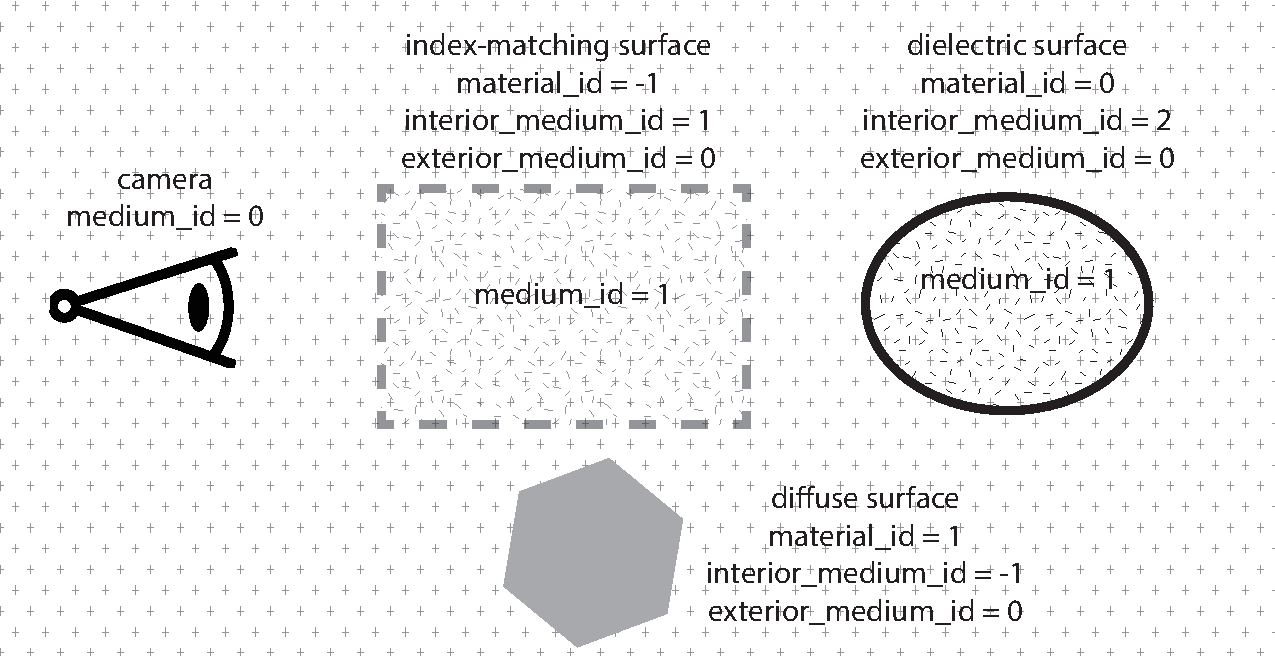
\includegraphics[width=\linewidth]{imgs/media.pdf}
    \caption{Lajolla assumes that media are separated by closed surface boundaries. At the object surface, we store the ID of the interior and exterior media (if either of them is vaccum, set the ID to \lstinline{-1}). The outmost medium is specified at the camera (and can be accessed through \lstinline{camera.medium_id}). A surface can be \emph{index-matching} meaning that light just pass through without changing direction or losing energy. In this case, the \lstinline{material_id} of the surface is set to \lstinline{-1}. A surface can also be transmissive. In this case, it is assigned a transmissive material like \lstinline{roughdielectric}.}
    \label{fig:data_structure}
\end{figure}

\paragraph{The Medium struct in lajolla.} Lajolla's medium interface is for querying the media parameters $\sigma_a$, $\sigma_s$, phase function $\rho$, and the \emph{majorant} which is the upper bound of the extinction coefficient $\sigma_t = \sigma_a + \sigma_s$ -- we will need the majorant in our final renderer. 
\begin{lstlisting}[language=c++]
struct MediumBase {
    PhaseFunction phase_function;
};

struct HomogeneousMedium : public MediumBase {
    Spectrum sigma_a, sigma_s;
};

struct HeterogeneousMedium : public MediumBase {
    VolumeSpectrum albedo, density;
};

using Medium = std::variant<HomogeneousMedium, HeterogeneousMedium>;

/// the maximum of sigma_t = sigma_s + sigma_a over the whole space
Spectrum get_majorant(const Medium &medium, const Ray &ray);
Spectrum get_sigma_s(const Medium &medium, const Vector3 &p);
Spectrum get_sigma_a(const Medium &medium, const Vector3 &p);

inline PhaseFunction get_phase_function(const Medium &medium) {
    return std::visit([&](const auto &m) { return m.phase_function; }, medium);
}
\end{lstlisting}
You will need these functions to obtain the necessary quantities in the homeworks.

A \lstinline{HomogeneousMedium} should be straightforward: it contains constant $\sigma_a$ and $\sigma_s$.
We will talk more about \lstinline{HeterogeneousMedium} and \lstinline{PhaseFunction} later.

Lajolla assumes that the media are separated by surface boundaries (Figure~\ref{fig:data_structure}). It's up to the upstream user to make sure they are consistent to each other and the surfaces are closed (if they are not, the results are undefined).\footnote{Modern production volume renderers have paid special attention to make sure the renderers can handle all sorts of inputs, including nested volumes. See \href{here}{https://graphics.pixar.com/library/ProductionVolumeRendering/index.html} for more information.} 

In the scene file, each objects are marked with corresponding exterior and interior media:
\begin{lstlisting}[language=xml]
    <medium type="homogeneous" id="medium">
        <rgb name="sigmaA" value="0.5 0.5 0.5"/>
        <rgb name="sigmaS" value="0.0 0.0 0.0"/>
        <float name="scale" value="3"/>
    </medium>

    <shape type="sphere">
        <!-- ...  -->
        <ref name="exterior" id="medium"/>
    </shape>

    <sensor type="perspective">
        <!-- ... -->

        <ref id="medium"/>
    </sensor>
\end{lstlisting}

The \lstinline{Medium}s are stored in \lstinline{scene.media} which you can access through \lstinline{scene.media[medium_id]}. The \lstinline{intersection} routine in lajolla returns a \lstinline{PathVertex} object which contains relevant information of the intersection:
\begin{lstlisting}[language=c++]
struct PathVertex {
    Vector3 position;
    Vector3 geometry_normal;
    // ...
    int shape_id = -1;
    int primitive_id = -1; // For triangle meshes. This indicates which triangle it hits.
    int material_id = -1;

    // If the path vertex is inside a medium, these two IDs
    // are the same.
    int interior_medium_id = -1;
    int exterior_medium_id = -1;
};
\end{lstlisting}

\section{Single monochromatic absorption-only homogeneous volume}
\begin{figure}
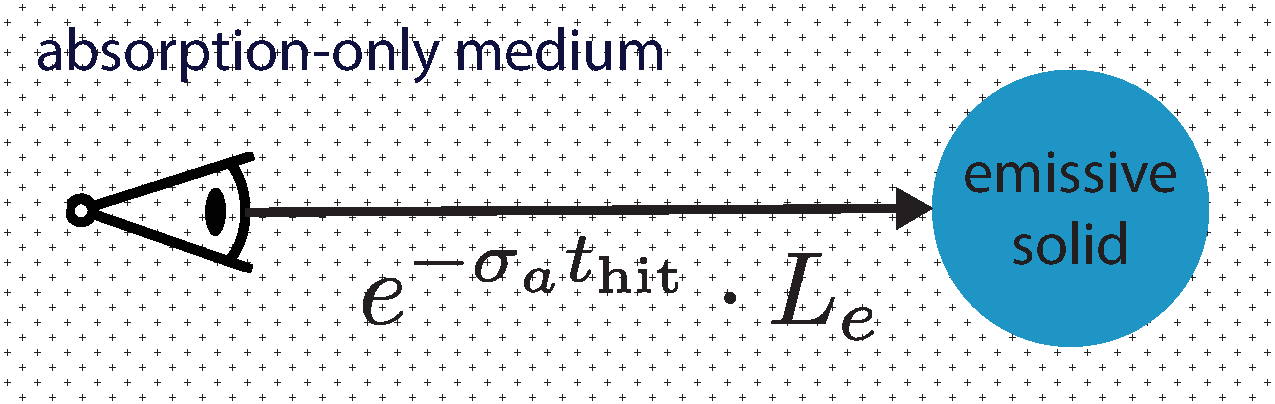
\includegraphics[width=\linewidth]{imgs/absorption_medium.pdf}
\caption{The setup of our first volumetric renderer.}
\label{fig:volpath1_illustration}
\end{figure}

Our first volume renderer will make four assumptions:
\begin{itemize}
    \item There is only a single, homogeneous ($\sigma_a$ and $\sigma_s$ are constants over space) volume.
    \item The volume does not scatter light: $\sigma_s = 0$.
    \item The surfaces in the scene only emit lights (with intensity $L_e$) and do not reflect/transmit lights.
    \item The volume is monochromatic: the three color channels of $\sigma_s$ and $\sigma_a$ have the same values.
\end{itemize}

Under these assumptions, the radiative transfer equation becomes
\begin{equation}
\frac{\mathrm{d}}{\mathrm{d}t} L_1(\mathbf{p}(t), \omega) = -\sigma_a L_1(\mathbf{p}(t), \omega),
\end{equation}
and we know $L_1(\mathbf{p}(t_{\text{hit}}), \omega) = L_e(\mathbf{p}(t_{\text{hit}}))$ where $t_{\text{hit}}$ is the distance between the origin of the ray and the emissive surface. 

This ordinary differential equation has a simple closed form:
\begin{equation}
L_1(\mathbf{p}(0), \omega) = \exp\left(-\sigma_a t_{\text{hit}} \right) L_e(\mathbf{p}(t_{\text{hit}})).
\end{equation}
Figure~\ref{fig:volpath1_illustration} illustrates the setup. In volume rendering the exponential term
$\exp\left(-\sigma_a t_{\text{hit}} \right)$ is often called the ``transmittance''.

Our rendering algorithm (that generates a sample for a pixel) is as follows (in Python-style pseudo code).
\begin{lstlisting}[language=python]
def L(screen_pos, rng):
  camera_ray = sample_primary(camera, screen_pos, rng)
  isect = intersect(scene, camera_ray)
  if isect:
    transmittance = exp(-sigma_a * t)
    Le = 0
    if is_light(isect):
      Le = isect.Le
    return transmittance * Le
  return 0
\end{lstlisting}

\begin{figure}
\centering
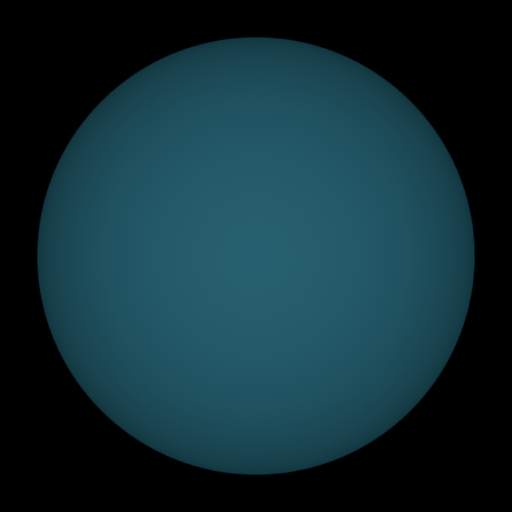
\includegraphics[width=0.5\linewidth]{imgs/volpath_1.png}
\caption{How Figure~\ref{fig:volpath1_illustration} would be rendered like.}
\label{fig:volpath1}
\end{figure}

\paragraph{Task (10\%).} You will implement the algorithm above in the \lstinline{vol_path_tracing_1} function in \lstinline{vol_path_tracing.h}. You might want to first look at the surface path tracing code in \lstinline{path_tracing.h} to understand lajolla's API better. Test your rendering using the scene \lstinline{scenes/volpath_test/volpath_test1.xml}. You should get an image that looks like Figure~\ref{fig:volpath1}.

\paragraph{Ray differentials.} In the surface path tracer, lajolla uses ray differential for texture lookup. Determining ray differentials for volumetric scattering is actually an unsolved problem. For this homework, we will just disable ray differentials by setting it to 0:
\begin{lstlisting}[language=c++]
RayDifferential ray_diff = RayDifferential{Real(0), Real(0)};
\end{lstlisting}

\paragraph{Environment maps.} Throughout the homework, we will assume there is no environment map in the scene. 

\paragraph{Question(s) (5\%).} Change the absorption parameters to zero in \lstinline{scenes/volpath_test/volpath_test1.xml}. What do you see? Why?

\section{Single monochromatic homogeneous volume with absorption and single-scattering, no surface lighting}
\begin{figure}
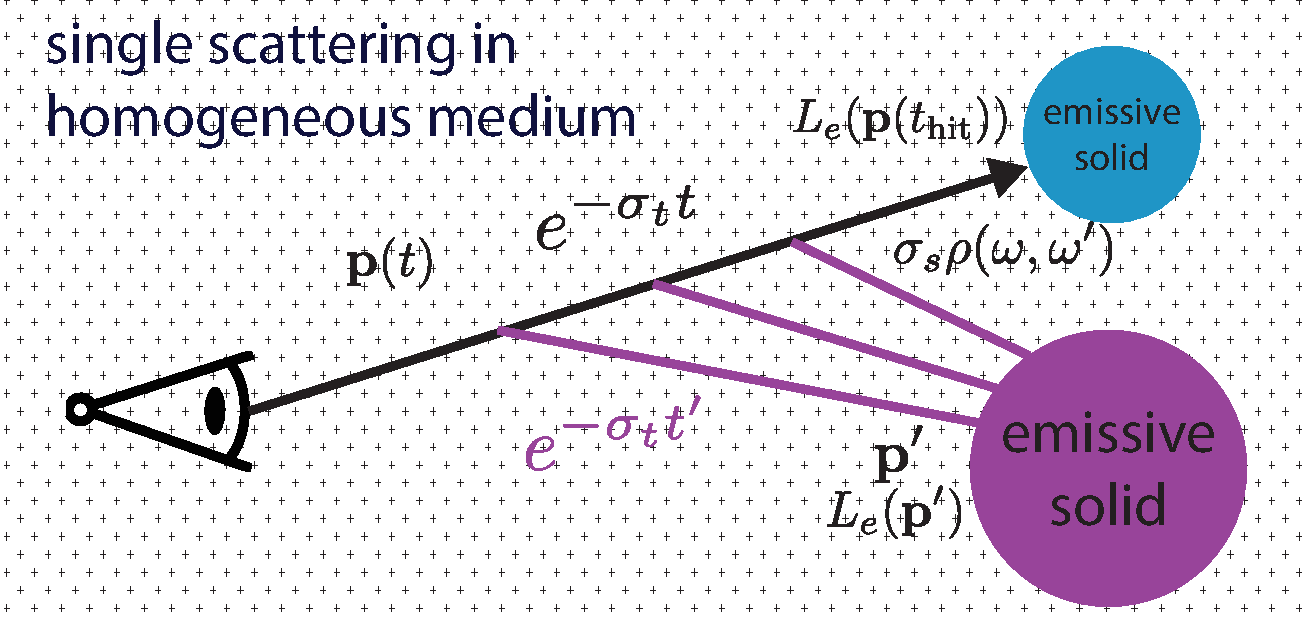
\includegraphics[width=\linewidth]{imgs/single_scattering.pdf}
\caption{The setup of our second volumetric renderer. Light can now scatter inside the medium once and we need to account for the phase function $\rho$ and the extra transmittance $\exp{-\sigma_t t'}$ We need to integrate over the ray to account for all scattering.}
\label{fig:volpath2_illustration}
\end{figure}

Our next renderer adds single scattering to the volume (Figure~\ref{fig:volpath2_illustration}). We still assume:
\begin{itemize}
    \item There is only a single, homogeneous ($\sigma_a$ and $\sigma_s$ are constants over space) volume.
    \item The surfaces in the scene only emit lights (with intensity $L_e$) and do not reflect/transmit lights.
    \item The volume is monochromatic: the three color channels of $\sigma_s$ and $\sigma_a$ have the same values.
    \item Light only scatter (changes direction) once in the volume.
\end{itemize}

Now we need to solve the full radiative transfer equation (Equation~\ref{eq:rte}), except the spherical integral only recurse once:
\begin{equation}
L_{\text{scatter}1}(\mathbf{p}, \omega) = \int_{\mathcal{M}} \rho(\mathbf{p}(t), \omega, \omega') L_e(\mathbf{p}', \omega) \exp\left(-\sigma_t \left\| \mathbf{p}(t) - \mathbf{p}' \right\|\right) \frac{\left| \omega' \cdot \mathbf{n}_{\mathbf{p}'} \right|}{{\left\| \mathbf{p}(t) - \mathbf{p}' \right\|}^2} \text{visible}(\mathbf{p}(t), \mathbf{p}') \mathrm{d}\mathbf{p}',
\end{equation}
instead of integrating over the sphere $S^2$, we apply a change of variable to integrate over the scene manifold $\mathcal{M}$ over all points on surfaces $\mathbf{p}'$. $\frac{\left| \omega' \cdot \mathbf{n}_{\mathbf{p}'} \right|}{{\left\| \mathbf{p}(t) - \mathbf{p}' \right\|}^2} \text{visible}(\mathbf{p}(t), \mathbf{p}')$ is the Jacobian of the transformation and $\omega' = \frac{\mathbf{p}' - \mathbf{p}(t)}{\left\| \mathbf{p}' - \mathbf{p}(t) \right\|}$. $\exp\left(-\sigma_t \left\| \mathbf{p}(t) - \mathbf{p}' \right\|\right)$ is the transmittance between $\mathbf{p}(t)$ and $\mathbf{p}'(t)$ that represents energy loss due to absorption and out-scattering (hence it uses the extinction coefficient $\sigma_t = \sigma_a + \sigma_s$ instead of $\sigma_a$ or $\sigma_s$). $s1$ stands for ``scattering once''.

The radiative transfer equation is then
\begin{equation}
\frac{\mathrm{d}}{\mathrm{d}t} L_2(\mathbf{p}(t), \omega) = -\sigma_t L_2(\mathbf{p}(t), \omega) + \sigma_a L_e(\mathbf{p}(t), \omega) + \sigma_s L_{\text{scatter}1}(\mathbf{p}, \omega).
\label{eq:rte_single_scattering}
\end{equation}

We no longer have a simple closed-form solution and have to resort to Monte Carlo sampling. To make the differential equation more familiar to us who are more used to Monte Carlo rendering, let's convert the equation above into an integral:
\begin{equation}
L_2(\mathbf{p}(0), \omega) = \int_{0}^{t_{\text{hit}}} \exp\left(-\sigma_t t \right) \sigma_s L_{\text{scatter}1}(\mathbf{p}, \omega) \mathrm{d}t + \exp\left(-\sigma_t t_{\text{hit}} \right) L_e(\mathbf{p}(t_{\text{hit}}))
\label{eq:rte_single_scattering_integral_form}
\end{equation}

To sample this integral, we importance sample the transmittance $\exp\left(-sigma_t t\right)$. To do this we need to sample $t$ such that $p(t) \propto \exp\left(-\sigma_t t\right)$. This can be done by standard inverse tranform sampling. We first integrate $\exp\left(-\sigma_t t \right)$:
\begin{equation}
\int_{0}^{t} \exp\left(-\sigma_t s\right) \mathrm{d}s = -\frac{exp(-\sigma_t * t)}{\sigma_t} + \frac{1}{\sigma_t}.
\end{equation}
We thus know that $p(t) = \sigma_t\exp\left(-\sigma_t t\right)$ (setting $t \rightarrow \infty$ we can get our normalization factor). Integrating $p(t)$ to get the CDF we get
\begin{equation}
T_{\text{exp}}^{-1}(t) = -\exp\left(-\sigma_t * t\right) + 1 = u.
\end{equation}
Inverting $T_{\text{exp}}^{-1}$ we get
\begin{equation}
t = \frac{\log\left(1 - u\right)}{-\sigma_t}.
\end{equation}

Now, note that our integral is only in $[0, t_{\text{hit}}]$. Our sampling above can generate $t > t_{\text{hit}}$. In this case, we hit a surface and account for the surface emission $L_e(\mathbf{p}(t_{\text{hit}}))$ in Equation~\ref{eq:rte_single_scattering_integral_form}. We need to account for the probability of that happen:
\begin{equation}
P(t \geq t_{\text{hit}}) = \int_{t_{\text{hit}}^{\infty} \sigma_t\exp\left(-\sigma_t t\right)} = \exp\left(-sigma_t * t_{\text{hit}}\right)
\end{equation}

Thus our rendering algorithm (that generate a sample for a pixel) looks like this:
\begin{lstlisting}[language=python]
def L(screen_pos, rng):
  camera_ray = sample_primary(camera, screen_pos, rng)
  isect = intersect(scene, camera_ray)
  if isect:
    u = next(rng) # u \in [0, 1]
    t = (1 - u) / sigma_t
    if t < isect.t_hit:
        trans_pdf = exp(-sigma_t * t) * sigma_t
        transmittance = exp(-sigma_t * t)
        # compute L_s1 using Monte Carlo sampling
        p = camera_ray.org + t * camera_ray.dir
        # Equation 7
        L_s1_estimate, L_s1_pdf = L_s1(p, sample_point_on_light(rng))
        return (transmittance / trans_pdf) * (L_s1_estimate / L_s1_pdf)
    else:
        # hit a surface, account for surface emission
        trans_pdf = exp(-sigma_t * isect.t_hit)
        transmittance = exp(-sigma_t * isect.t_hit)
        Le = 0
        if is_light(isect):
          Le = isect.Le
        return (transmittance / trans_pdf) * Le
  return 0
\end{lstlisting}

\begin{figure}
\centering
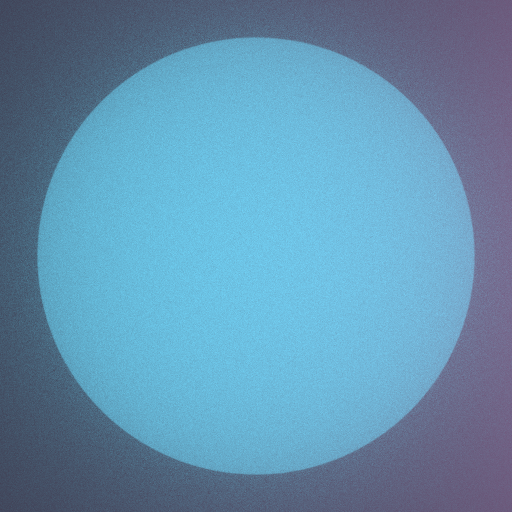
\includegraphics[width=0.5\linewidth]{imgs/volpath_2.png}
\caption{How a scene like the setup in Figure~\ref{fig:volpath2_illustration} would be rendered like. Now there is scattering, the area surrounding the solid sphere can have non-zero radiance.}
\label{fig:volpath2}
\end{figure}

\paragraph{Task (10\%).} You will implement the algorithm above in the \lstinline{vol_path_tracing_2} function in \lstinline{vol_path_tracing.h}. For evaluating the phase function $\rho$, use the \lstinline{eval} function in \lstinline{phase_function.h}.
Test your rendering using the scene \lstinline{scenes/volpath_test/volpath_test2.xml}. You should get an image that looks like Figure~\ref{fig:volpath2}. Note that the rendered image will be a bit noisy even a high sampling count. This is expected, since we are not importance sampling the geometry term $\frac{\left| \omega' \cdot \mathbf{n}_{\mathbf{p}'} \right|}{{\left\| \mathbf{p}(t) - \mathbf{p}' \right\|}^2} \text{visible}(\mathbf{p}(t), \mathbf{p}')$ along $t$. Such importance sampling scheme is called the \emph{equiangular sampling}~\cite{Kulla:2012:IST} (or \emph{track-length estimator} in nuclear engineering~\cite{Rief:1984:TLE}). Equiangular sampling is out of the scope for this homework, but you're free to implement it!

\paragraph{Question(s) (5\%).} Play with the parameters $\sigma_s$ and $\sigma_a$, how do they affect the final image? Why? (Note that we assume monochromatic volumes, so don't set the parameters to be different for each channel.)

\paragraph{Bonus (25\%).} Implement the \emph{equiangular sampling}~\cite{Kulla:2012:IST} sampling strategy. Potentially combine it with the transmittance sampling using multiple importance sampling. (I do not recommend you implement this until you've finished the whole homework.)

\section{Multiple monochromatic homogeneous volumes with absorption and multiple-scattering using only phase function sampling, no surface lighting}
\begin{figure}
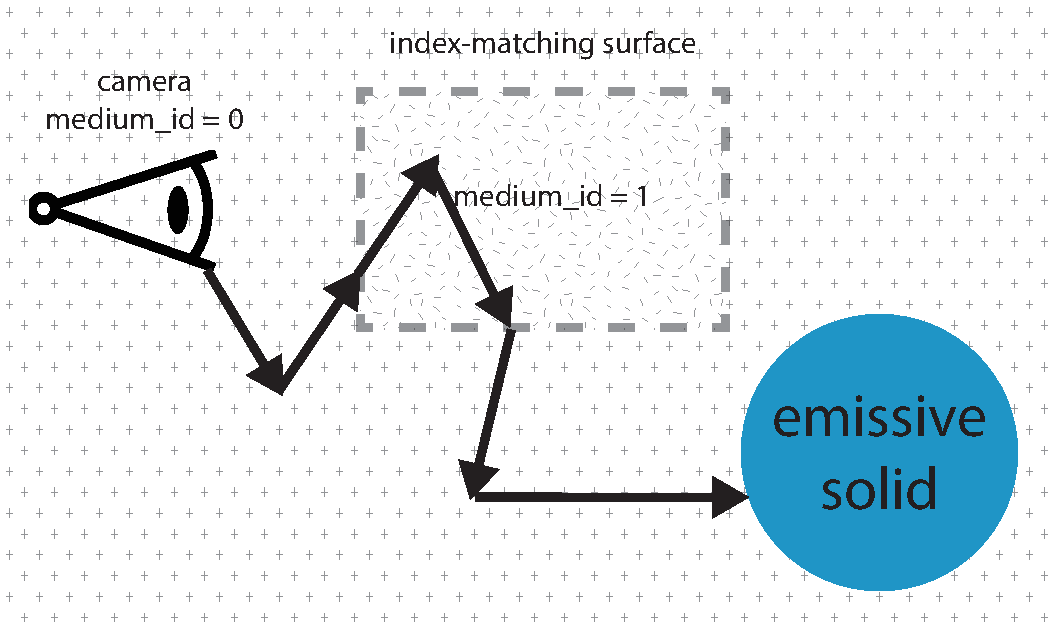
\includegraphics[width=\linewidth]{imgs/multiple_scattering.pdf}
\caption{Setup of our third volumetric renderer.}
\label{fig:volpath3_illustration}
\end{figure}
Our next volumetric path tracer would start to be a bit complicated. This time we will consider multiple scattering between multiple volumes (Figure~\ref{fig:volpath3_illustration}). We make the following assumptions:
\begin{itemize}
    \item There are multiple homogeneous ($\sigma_a$ and $\sigma_s$ are constants over space) volumes.
    \item The surfaces in the scene only emit lights (with intensity $L_e$) and do not reflect/transmit lights.
    \item The volume is monochromatic: the three color channels of $\sigma_s$ and $\sigma_a$ have the same values.
    \item Light can scatter (changes direction) multiple times in the volume, but we only sample the scattering by sampling the phase function $\rho$.
\end{itemize}

Under this assumption, our volumetric integral becomes:
\begin{equation}
L_3(\mathbf{p}(0), \omega) = \int_{0}^{t_{\text{hit}}} \exp\left(-\sigma_t t \right) \sigma_s L_{\text{scatter}}(\mathbf{p}, \omega) \mathrm{d}t + \exp\left(-\sigma_t t_{\text{hit}} \right) L_e(\mathbf{p}(t_{\text{hit}})),
\label{eq:rte_multiple_scattering_integral_form}
\end{equation}

where $L_{\text{scatter}}$ is recursive:
\begin{equation}
L_{\text{scatter}}(\mathbf{p}, \omega) = \int_{S^2} \rho(\mathbf{p}(t), \omega, \omega') L_3(\mathbf{p}(t), \omega') \mathrm{d}\omega'.
\end{equation}

Our strategy of sampling the integral $L_3$ is as follows: we first generate a distance $t$ by sampling the transmittance as previous. If $t < t_{\text{hit}}$, we need to evaluate $L_{\text{scatter}}$. We do so by sampling the phase function $\rho$ for a direction $\omega'$. We then sample the next distance for evaluating the $L_3$ inside the $S^2$ integral. If we hit a surface ($t' \geq t'_{\text{hit}}$ for some distance $t'$ along our sampling), we include the emission $L_e$ and terminate.

\paragraph{Number of bounces.} We use the \lstinline{scene.options.max_depth} parameter to control the number of bounces. If \lstinline{max_depth = -1}, then we can bounce infinite amount of time. Otherwise, a light path can have at most \lstinline{max_depth + 1} vertices, including the camera vertex and the light vertex. \lstinline{max_depth = 2} corresponds to the single scattering case in the previous section.

\paragraph{Index-matched surfaces.} Sometimes we will hit surfaces that have no materials assigned (\lstinline{material_id = -1}). For these surfaces, we need to pass through them. Passing through an index-matched surface counts as one bounce.

\paragraph{Russian roulette.} We use the \lstinline{scene.options.rr_depth} to control the Russian roulette behavior. We initialize Russian roulette when a light path has \lstinline{rr_depth + 1} vertices.

The pseudo code looks like this:
\begin{lstlisting}[language=python]
def L(screen_pos, rng):
  ray = sample_primary(camera, screen_pos, rng)
  current_medium = camera.medium

  current_path_throughput = 1
  radiance = 0
  bounces = 0
  while True
    scatter = False
    isect = intersect(scene, ray)
    # isect might not intersect a surface, but we might be in a volume
    transmittance = 1
    trans_pdf = 1
    if current_medium:
      # sample t s.t. p(t) ~ exp(-sigma_t * t)
      # compute transmittance and trans_pdf
      # if t < t_hit, set scatter = True
      # ...
      ray.org = ray.org + t * ray.dir
    
    current_path_throughput *= (transmittance / trans_pdf)
    if not scatter:
      # reach a surface, include emission
      radiance += current_path_throughput * Le(isect)

    if bounces == max_depth - 1 and max_depth != -1:
      # reach maximum bounces
      break

    if not scatter and isect:
      if isect.material_id == -1:
        # index-matching interface, skip through it
        current_medium = update_medium(ray, isect)
        continue

    # sample next direct & update path throughput
    if scatter:
      next_dir = sample_phase_function(-ray.dir, rng)
      current_path_throughput *=
        (phase_function(-ray.dir, next_dir) / sample_phase_pdf(-ray.dir, next_dir)) * sigma_s
    else:
      # Hit a surface -- don't need to deal with this yet
      break
    
    # Russian roulette
    rr_prob = 1
    if (bounces >= rr_depth):
      rr_prob = min(current_path_throughput, 0.95)
      if next(rng) > rr_prob:
        break
      else:
        current_path_throughput /= rr_prob
    
    bounces += 1

  return radiance
\end{lstlisting}

\begin{figure}
\centering
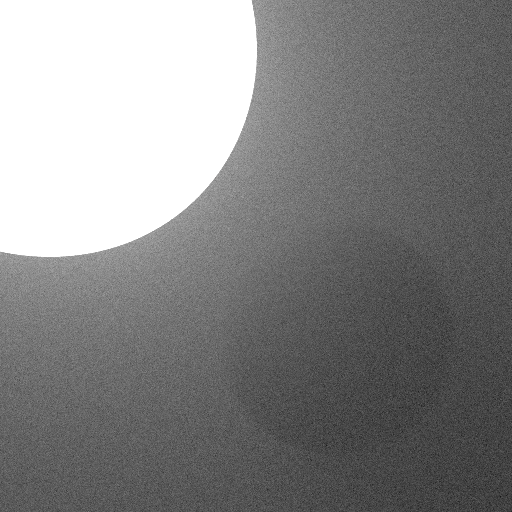
\includegraphics[width=0.5\linewidth]{imgs/volpath_3.png}
\caption{How Figure~\ref{fig:volpath3_illustration} would be rendered like. Left top is a light source, and bottom right is an volume with index-matched interface.}
\label{fig:volpath3}
\end{figure}

\paragraph{Task (10\%).} You will implement the algorithm above in the \lstinline{vol_path_tracing_3} function in \lstinline{vol_path_tracing.h}. For sampling the phase function $\rho$, use the \lstinline{sample_phase_function} and \lstinline{pdf_sample_phase} functions in \lstinline{phase_function.h}.
Test your rendering using the scene \lstinline{scenes/volpath_test/volpath_test3.xml}. You should get an image that looks like Figure~\ref{fig:volpath3}. Again, the image can be a bit noisy since we have not implemented next event estimation.

\paragraph{Question(s) (5\%).} Play with the parameters $\sigma_s$, $\sigma_a$ of different volumes, and change \lstinline{max_depth}, how do they affect the final image? Why?


\bibliographystyle{plain}
\bibliography{refs}

\end{document}